\begin{anexosenv}

\partanexos
\chapter{Regras Originais do Jogo \textit{Big Points}}

	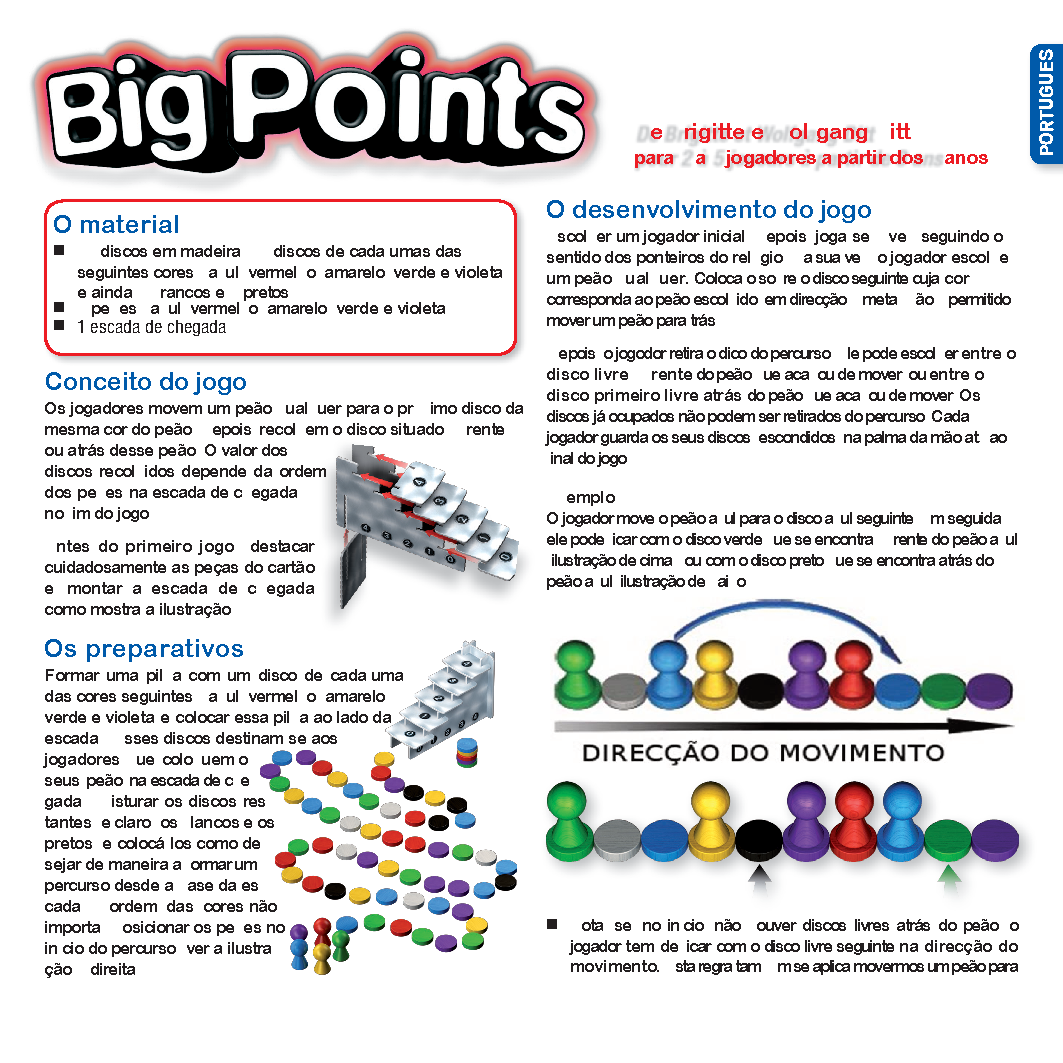
\includepdf[pages={-}]{BigPoints_rules.pdf}


%
%\chapter{Processo de Renderização}
%\label{renderpipe}


%	O processo de geração de gráficos tridimensionais em computadores tem início com a criação de cenas. Uma cena é composta por objetos, que por sua vez são compostos por primitivas geométricas (como triângulos, quadrados, linhas, entre outros) que são constituídas de vértices, estabelecendo a geometria. Todos estes vértices seguem um processo similar de processamento para formarem uma imagem na tela.  Este processo é mostrado na Figura \ref{pipeline} e as próximas seções detalham cada uma das etapas ilustradas.


%\section{Processamento dos Dados dos Vértices}

%	A etapa de Processamento dos Dados dos Vértices é responsável por configurar os objetos utilizados para renderização com um \textit{shader} específico, dependendo da técnica de renderização de modelos tridimensionais utilizada. Uma destas técnicas é a utilização de um \textit{vertex array object}, que descreve o modelo tridimensional por meio de uma lista de vértices e uma lista de índices. Na Figura \ref{quadrado}, tem-se dois triângulos e quatro vértices definidos (dois vértices são compartilhados). Assim, pode-se definir um vetor com os vértices [v0, v1, v2, v3] e um vetor de índices [0, 3, 1, 0, 2, 3], que determina a ordem em que os vértices devem ser renderizados.
\end{anexosenv}
